\documentclass[12pt,a5paper]{article}

\usepackage[T1]{fontenc} % font encoding, lubab õ tähte kasutada
\usepackage[utf8]{inputenc} % oleme siiski 21. sajandis, vajadusel on ka olemas utf8x
\usepackage{lmodern} % lmodern ja micrtype käivad käsikäes, teeb teksti ilusamaks
\usepackage{microtype}
\usepackage[estonian]{babel} % eesti keele poolitamisreeglid jpm
\usepackage[per = fraction, expproduct=cdot, decimalsymbol=comma, inter-unit-product=\cdot]{siunitx} % http://www.bakoma-tex.com/doc/latex/siunitx/siunitx.pdf
\usepackage{graphicx} 
\usepackage{wrapfig}
\usepackage{tikz}
\usepackage[european]{circuitikz}
\tikzset{component/.style={draw,thick,circle,fill=white,minimum size =0.75cm,inner sep=0pt}}
\usepackage{amsmath,amssymb} 
\usepackage{amsfonts}
\usepackage{epstopdf} %minul on vaja, et .eps pilte saada
%paneme kõik mõõdud paika
\topmargin=-3.0cm \textheight=19cm \textwidth=12.9cm
\oddsidemargin=-1.5cm  \evensidemargin=-1.5cm
\setlength{\parindent}{0pt} \setlength{\parskip}{6pt} \sloppy
\relpenalty=10000 \binoppenalty=10000 % Tekstisisestes valemites reavahetusi ärgu olgu
\pagestyle{empty} % ilma leheküljenumbrita
\newcommand{\numb}[1]{\vspace{5pt}\textbf{\large #1}}
\newcommand{\nimi}[1]{(\textsl{\small #1})}
\newcommand{\punktid}[1]{(\emph{#1~p.})}
\newcounter{ylesanne}
\newcommand{\yl}[1]{\addtocounter{ylesanne}{1}\numb{\theylesanne.} \nimi{#1} \newblock{}}
\newcommand{\autor}[1]{\emph{ Autor: #1}}
\newcommand{\D}{\textrm{d}}

\begin{document}

\begin{center}
\textbf{\Large Eesti koolinoorte 66. füüsikaolümpiaad} \vspace{3pt}

\emph{06. aprill 2019. a. Lõppvoor.}

\emph{Gümnaasiumi ülesanded (10. - 12. klass)}

\emph{Palun kirjutage iga ülesande lahendus eraldi lehele!}

\end{center}

\yl{AUTOD}
Kaks autot sõidavad teineteise poole. Esimese auto kiirus $v_1=\SI{80}{km/h}$ ning teise auto kiirus $v_2 = \SI{100}{km/h}$. Autod märkavad teinetest, kui nende vahekaugus $s=\SI{600}{m}$ ning hakkavad samal hetkel pidurdama. Autod jäävad seisma samal hetkel, vahetult enne kokkupõrget. Kui kaua võttis autodel aega peatumine? \punktid{6}

\yl{SAUNAUKS}
Juku istub saunas ja viskab saunakerisele vett. Tekkinud leilist läheb saunauks lahti. Arvutage, kui suur peaks olema hõõrdejõu moment $\tau$ saunaukse hingedes, et $V_v=\SI{200}{ml}$ vett korraga kerisele visates saunauks lahti ei läheks? Sauna mõõtmed on $300 \times 250 \times 240$ cm, sauna ukse mõõtmed $70 \times 190$ cm. Eeldada, et aurustumine toimub nii kiiresti, et õhk ei jõua läbi pilude saunast välja minna. Universaalne gaasikonstant $R=\SI{8,314}{J/(mol \cdot K)}$, vee molaarmass $\mu=\SI{18}{g/mol}$ ja vee tihedus $\rho = \SI{1}{g/cm^3}$. \punktid{8}

\begin{wrapfigure}[12]{r}{0.37\textwidth}
  \vspace{-28pt}
  \begin{center}
  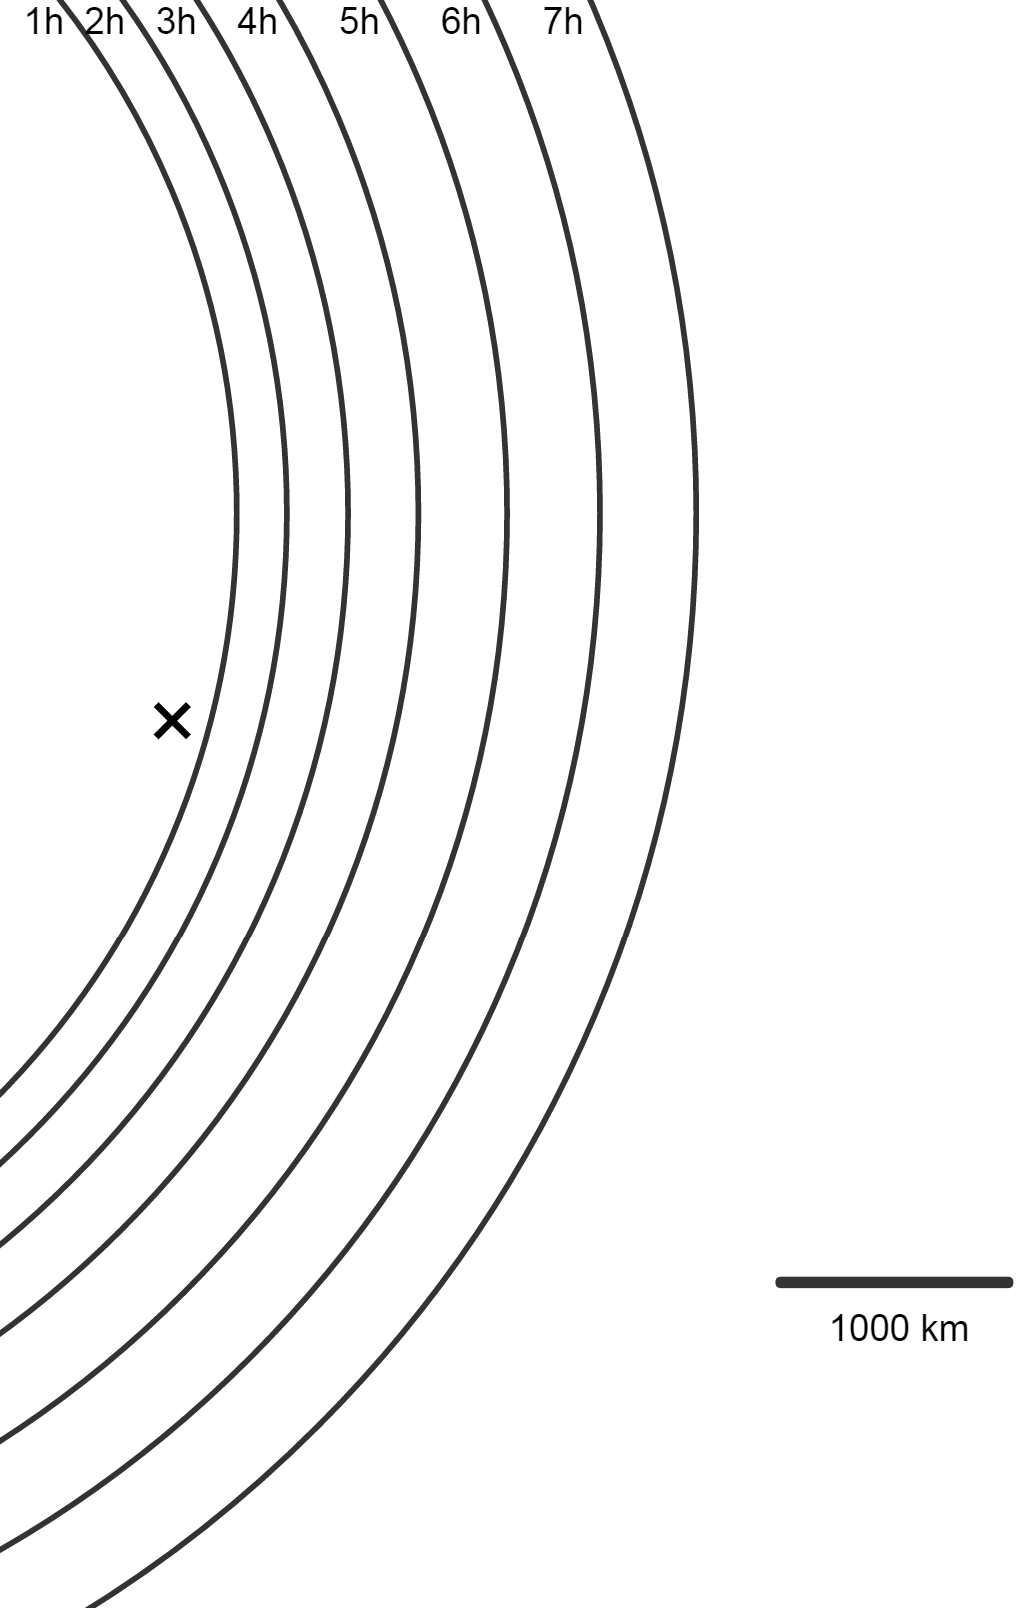
\includegraphics[scale=0.2]{LennukProblem.png}
  \end{center}
  \vspace{-20pt}
\end{wrapfigure}


\yl{LENNUK} Joonisel on lennuki algne asukoht märgitud ristiga. Iga tunni järel mõõdeti lennuki kaugust fikseeritud punktist. Saadud kaugused on joonisel märgitud ringjoonena mõõtepunkti ümber. Konstrueerige kõikvõimalikud lennuki trajektoorid $\SI{7}{h}$ jooksul, kui on teada, et pärast starti lendas lennuk $\SI{4}{h}$ otse, muutis seejärel suunda ning lendas ülejäänud aja samuti otse. Eeldada, et lennuki kiirus maapinna suhtes oli ühtlaselt $\SI{500}{km/h}$. Lahendus esitada lisalehel.
\textit{Märkus.} Suuna muutus võis olla ka väga väike. \punktid{8}
\newpage

\yl{KONVEIER} Sile metallplaat pikkusega $l$ sõidab konveieril. Konveier koosneb kahest osast ning kummalgi osal on oma sile konveierilint. Mõlema lindi pikkus on $x$, kuid esimene lint liigub kiirusega $v_1$ ning teine kiirusega $v_2$. Algasendis on plaat esimese lindi alguses nii, et plaat asub täielikult esimesel konveierilindil ning plaadi tagumine serv ühtib esimese lindi algusega. Lõppasendis on plaat teise lindi lõpus nii, et plaat asub täielikult teisel konveierilindil ning plaadi esimene serv ühtib teise lindi lõpuga. Leida aeg $t$, mis kulub plaadil algasendist lõppasendisse jõudmiseks. Hõõrdetegur plaadi ja esimese konveierilindi vahel on $\mu_{1}$ ning plaadi ja teise konveierilindi vahel $\mu_{2}$. Eeldada, et üleminekukohas on vahe konveierilintide vahel tühiselt väike ning aeg, mis kulub plaadi kiiruse muutumiseks üleminekukohas, on tühiselt väike võrreldes koguajaga. \punktid{8}



\begin{wrapfigure}{r}{0.38\textwidth}
  \vspace{-25pt}
  \begin{center}
    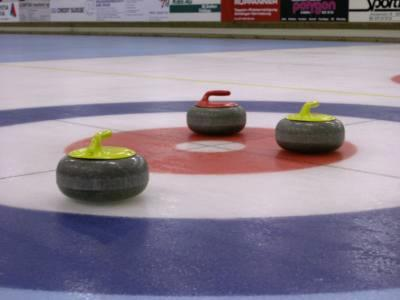
\includegraphics[width=0.4\textwidth]{Curling_stones.jpg}
    % Pildi allikas Wikimedia Commons https://upload.wikimedia.org/wikipedia/commons/4/4f/Curling_stones.jpg
  \end{center}
  \vspace{-20pt}
\end{wrapfigure}

\yl{JÄÄKEEGEL} Jääkeegel ehk kurling on talispordimäng, mille eesmärgiks on enda meeskonna kivide libistamine jääväljakule märgitud märklaua keskkohale võimalikult lähedale. Sealjuures on lubatud enda kividega vastase kivisid eemale tõugata. Vaatamegi olukorda, kus vastasel on õnnestunud üks kivi täpselt märklaua keskele libistada. Kui suure kiirusega $v_0$ peaks oma kiviga vastase kivi tabama, et pärast vastase kivi eemaletõukamist jääks see ise täpselt märklaua keskele? Jääkeeglikivid on võrdse massiga ning läbimõõduga $D=\SI{29}{cm}$. Hõõrdetegur jää ja kivide vahel on $\mu = \num{0.02}$ ning kividevahelisel põrkel muundub soojuseks $\eta=40\%$ esialgsest kineetilisest energiast. Raskuskiirendus $g=\SI{9.8}{m/s^2}$.
\punktid{10}

\yl{LÕKS} Kuulike massiga $m$ ja laenguga $q$ sisenes läbi väikse augu silindrisse, mida täidab teljesihiline homogeenne magnetväli induktsiooniga $B$. Sisenemishetkel oli kuulikese kiirus radiaalsihiline. Kuulike väljus silindrist sama augu kaudu peale kahte absoluutselt elastset põrget silindri seintega. Kui kaua viibis kuulike silindris? \punktid{10}

\vspace{-5pt}

\begin{wrapfigure}[4]{r}{0.45\textwidth}
  \vspace{-15pt}
  \begin{center}
  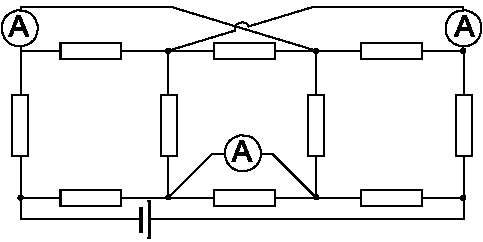
\includegraphics[scale=0.65]{3ruutu}
  \end{center}
  \vspace{-20pt}
\end{wrapfigure}

\newpage

\yl{3 RUUTU} Toodud skeemis on kõigi takistite takistus kolm oomi, patarei pinge on 48 volti. Leidke ampermeetrite näidud. \punktid{10}

\vspace{25pt}


\yl{KÄRBES} Kärbes lendab läätse peateljega paralleelselt, teljest kaugusel $a$, läätse suunas konstantse kiirusega $v$ alustades suurest kaugusest ja lõpetades läätse juures. Läätse fookuskaugus on $f$. Milline on selle lennu jooksul kärbse minimaalne kiirus tema kujutise suhtes? \punktid{12}

\yl{NIIT JA POOLSFÄÄR} Millise kogulaengu $Q$ indutseerib peenikese juhtme abil maandatud kerale, mille raadius on $R$, peenest traadist rõngas raadiusega $r$, mis kannab laengut $q$, kui kera ja rõnga keskpunktide vahekaugus on $d$ ning kera keskpunkt asub rõnga sümmeetriateljel? Maandamisjuhtme mahtuvus on tühiselt väike. \punktid{12}

\yl{PÖÖRDUV ELEKTRIVÄLI} Elektriväli $\vec E$ muudab perioodiga $4T$ oma suunda pöördudes $x-y$-tasandis iga 
ajavahemiku $T$ möödudes hüppeliselt $\SI{90}\degree$ päripäeva. Seega, kui $t$ tähistab aega 
ning $\hat x$ ja $\hat y$ tähistavad vastavalt $x$- ja $y$-telje sihilisi ühikvektoreid,  siis ajavahemikel
\begin{align*}
4nT\le &t < 4nT+T \;\; & \vec E&=E_0\hat x,\\
4nT+T\le &t < 4nT+2T   & \vec E&=-E_0\hat y,\\
4nT+2T\le &t < 4nT+3T  & \vec E&=-E_0\hat x \;\;\mbox{ja}\\
4nT+3T\le &t < 4nT+4T & \vec E&=E_0\hat y.
\end{align*}

On teada, et osake massiga $m$ ja laenguga $q$ liigub perioodiliselt, st mööda kinnist trajektoori; visandage selle osakese 
trajektoor $x-y$-tasandis ja leidke trajetoori $x$-telje sihiline läbimõõt. \punktid{12}

\end{document}